\documentclass[conference]{IEEEtran}
\IEEEoverridecommandlockouts
% The preceding line is only needed to identify funding in the first footnote. If that is unneeded, please comment it out.
\usepackage{cite}
\usepackage{algorithmic}
\usepackage{graphicx}
\usepackage{textcomp}
\usepackage{amsmath}
\usepackage[sc]{mathpazo}
\usepackage{datetime}
\usepackage{graphicx, wrapfig, subcaption, setspace, booktabs}
\usepackage[T1]{fontenc}
\usepackage{fourier}
\usepackage{url, lipsum}
\usepackage{hyperref,bookmark}
\usepackage[T1]{fontenc}
\usepackage{amssymb}
\usepackage{makecell, multirow, tabularx}
\usepackage{listings}
\usepackage[ruled,linesnumbered,vlined]{algorithm2e}

\usepackage{float}
\usepackage{nomencl}
\usepackage{ifthen}

\renewcommand{\nomgroup}[1]{%
	\ifthenelse{\equal{#1}{P}}{\item[\textbf{Parameters}]}{%
		\ifthenelse{\equal{#1}{V}}{\item[\textbf{Variables \\}]}}
}
\makenomenclature
\def\BibTeX{{\rm B\kern-.05em{\sc i\kern-.025em b}\kern-.08em
    T\kern-.1667em\lower.7ex\hbox{E}\kern-.125emX}}
\begin{document}

\title{CO\textsubscript{2} Impact Electric Vehicle Charging on a Local Microgrid: a case study in Southern California }

\author{
	\IEEEauthorblockN{Luis Fernando Enriquez-Contreras\IEEEauthorrefmark{1}\IEEEauthorrefmark{2}, Matthew Barth\IEEEauthorrefmark{1}\IEEEauthorrefmark{2}, Sadrul Ula\IEEEauthorrefmark{2}}
	\IEEEauthorblockA{\IEEEauthorrefmark{1}\textit{Department of Electrical  and Computer Engineering} \\
		\textit{University of California, Riverside}\\
				Riverside, United States of America \\
				lenri001@ucr.edu, barth@ece.ucr.edu}
	\IEEEauthorblockA{\IEEEauthorrefmark{2}\textit{College of Engineering, Center for Environmental Research \& Technology} \\
		\textit{University of California, Riverside}\\
				Riverside, United States of America \\
				lenri001@ucr.edu, barth@ece.ucr.edu, sula@cert.ucr.edu}
}
\maketitle

\begin{abstract}

	In this paper, we evaluate a case study at the University of California, Riverside (UCR) that simulates different EV charging setups with their associated electric costs and CO\textsubscript{2}. The CO\textsubscript{2} are calculated with high resolution CAISO CO\textsubscript{2} emissions data in order to review the different emission levels from the different setups. Electric costs are also compared in order to see the different savings the consumer will have with the different setups. It was found that Level 2 charging has a minimal impact on electric costs and CO\textsubscript{2} emissions, which can be offsetted with EV pricing, and by replacing trips from internal combustion engine (ICE) vehicles. Level 3 charging does cause a higher output of emissions, it can double the demand costs by itself. While the CO\textsubscript{2} can be offset from the prevented ICE trips, a prevention of Level 3 charging during peak times must be implemented to prevent high demand costs.
	

\end{abstract}

\begin{IEEEkeywords}
micorgrids, demand response, CO\textsubscript{2} emissions, modelica, EV charging
\end{IEEEkeywords}


\section{Introduction}
    \subsection{Background}
	California is committed to reducing greenhouse gas emissions through various approaches. However, the two largest contributors to greenhouse gas emissions in California are transportation and electricity generation. In California, 18.84 \% percent of 2022 vehicle sales were electric, \cite{ev_sale_percentage} and the state plans on banning internal combustion engine vehicles by 2035 \cite{ice_ban}. At the same time, California is increasing the number of charging stations in the state, having over 13,737 stations \cite{ev_stations_CA}. Electric vehicle technology has improved, and new vehicles can charge in 20-60 minutes \cite{ev_stats}. This is due to Level 3 charging, which can be as high as 350 kilowatts (kW), as opposed to Level 2 charging, which is capped at 19 kW \cite{ev_stats}. While this innovation has led to a higher practicality for electric vehicles, it also leads to more difficulty for the owners of these chargers since they can create a tremendous amount of loads very quickly. Most Level 2 chargers consumers use are similar in load to an air conditioner. While California tries to increase clean energy penetration, it also needs to reduce the amount of GHG emissions produced by transportation through electrification. This leads to two conundrums: how will California add enough capacity for electrified transport, and how clean is the grid to minimize the amount of emissions associated with battery electric vehicles? One proposal to mitigate the strain on the grid is to keep electricity production and EV charging local by using microgrids. A microgrid is defined as: “‘a group of interconnected loads and distributed energy resources within clearly defined electrical boundaries that acts as a single controllable entity with respect to the grid. A microgrid can connect and disconnect from the grid to enable it to operate in both grid-connected or island-mode” As microgrids and EV chargers become ubiquitous, it is crucial to study the economic and environmental impacts EV charging, in particular fast charging, will have on microgrids.
  	\subsection{Literature Review}
  		In  \cite{himabindu2021analysis},   Electric Vehicle Charging Stations (EVCS) are analyzed under different solar irradiation conditions.   The study develops a demand and stochastic model, then performs a techno-economic assessment and analyzes the environmental impact of EVCS.  The authors conclude that EVCS with solar's optimal configuration  and investment costs are highly dependent on feed-in tariffs and  the solar irradiation of the area. The  CO\textsubscript{2} emissions were calculated on a per year basis, and do not deal with the variations of  CO\textsubscript{2} emissions within a single day.  Also, only energy charges were calculated with no demand costs calculations. \citen{yoon2017economic},  proposes a control algorithm is proposed that in different scenarios can minimize charging time or costs or maximize renewable energy use. The authors used a uniform distribution during peak times  to model the charging loads, with only Level 2 charging at 3.3 kW and no Level 3 charging. An EV charging model is proposed in \cite{purvins2018electric},  that load shifts charging events from high peak times to low peak times.  The authors found their current method does little to reduce peak load shaving, and solar production surplus may not be necessarily shifted to EVs due to their low availability at the time.  The dataset was limited to one week ], with four EVs in a system with 10 buildings.  In \cite{Khemir}, the authors run multiple scenarios with different self consumption rates, first comparing scenarios and then calculating emissions for each scenario.. The CO\textsubscript{2} emissions are calculated from whole life-cycle CO \textsubscript{2}  emissions without a high time resolution.  \cite{huang2023multi} uses the Non-dominated Sorting Genetic Algorithm-
  		II (NSGA-II) to analyze 4 different responses with 0 \% 10 \% 20 \% 30\%  EV penetration and a Monte Carlo load profile.  Results were remarkable, however CO\textsubscript{2} calculations were not explained. and the specific impacts of  Level 2 vs Level 3 charging were not shown.  \cite{tan2020multi} analyzes IEEE  9 and 14 nodes  that forecast the EV loads one day ahead.  The author use multiple microgrids to balance out EV charging within the system.  Multi-objective energy management of multiple microgrids is used to orchestrate the operation.
  		
  		This paper's analyzes the impacts different Level 2 and Level 3 charging have on the behavior of microgrids and the associated electric costs and CO\textsubscript{2} emissions in southern California. The simulation is run in open Modelica rather than being a purely calculated model. This paper also uses a higher time resolution data than most to calculate the CO\textsubscript{2} emissions every 15 minutes.
    \subsection{Peak Shaving Strategy}
       		Peak shaving is a standard method for reducing high-demand charges. Since demand charges are based on only the maximum value over the entire month, we assume the consumer wants to minimize the demand charges as much as possible. Our algorithm is based solely on cost savings for a typical microgrid. During peak-shaving, the algorithm looks at the amount of power being imported, if there is enough energy, and if the batteries can mitigate a fraction of that or the total amount.  
    \subsection{CO\textsubscript{2} Emissions}
        	Our microgrid's solar production greatly overlaps with the local solar energy production within the larger grid.  With a BESS, we can utilize renewable energy during peak times and at night. In this scenario, the control algorithm is economically based since we want to see how EV charging aligns with actual CO\textsubscript{2} emission outputs.  While the micorgrid does not produce any direct CO\textsubscript{2} emissions, but rather the indirect The simulation uses emission output calculations from CAISO for each time interval as a sum of all the powerplant CO\textsubscript{2} emissions (imports, natural gas, biogas, biomass, geothermal, coal) $\frac{\textsubscript{m}TON\textsubscript{CO\textsubscript{2}}}{hour}$. The CO\textsubscript{2} emissions output is divided by the amount of power produced (solar, wind, geothermal, biomass, biogas, small hydro, grid batteries, large hydro, imports, nuclear, coal ) in MW, which gives us an emissions rate of $\frac{\frac{\textsubscript{m}TON\textsubscript{CO\textsubscript{2}}}{hour}}{W}$ . This is multiplied with our 15-minute data kW, and a multiplier. The multiplier of  $\frac{1}{4000}$ converts kW into W and to address for the four 15 minute periods in an hour multiples by four.  This gives us an estimate of the amount of CO\textsubscript{2} emissions in \textsubscript{m}TON\textsubscript{CO\textsubscript{2}} for every 15 minutes that is summed together to give us the total for the entire period.  This method is similar to the one used in \cite{garrido2021dynamic}.  When the grid does not pull power from the grid or is sending power, the CO\textsubscript{2} emissions are assumed to be zero since we are using our solar energy.
\section{Simulation in OpenModelica}
    	OpenModelica is an open-source implementation of the Modelica programming language \cite{OpenModelica}. Modelica is a programming language that is designed for dynamic systems simulation \cite{ModelicaLanguage}. OMEdit is the GUI interface for OpenModelica, allowing the user to draw a system for simulation \cite{OMEdit}. The microgrid scenarios are simulated in OpenModelica using the Modelica buildings library.  Lawrence Berkeley National Laboratory created the Modelica buildings library for building and district energy and control systems \cite{ModelicaBuildingsLibrary}. However, its capability for energy storage systems, bi-directional inverter, solar, and HVAC modeling make it ideal for a microgrid simulation setup. This allows us to create scenarios that do not currently exist in our microgrid, like running a month with solar with the same load, or running the BESS control algorithm for different electric rates.  The power circuits are three-phase balanced circuits. The simulation of our case study microgrid is the grid-connected to the building netload. The model's net load is broken down into solar power, HVAC loads, regular building loads, electric vehicle chargers, and the BESS as shown in Figure \ref{fig:powersystemsetupfull}.
	\begin{figure}[H]
		\centering
		\includegraphics[width=1\linewidth]{Fig/power_system_setup_modelica}
		\caption{Microgrid Layout}
		\label{fig:powersystemsetupfull}
	\end{figure}
	\subsection{Validation}
		To ensure that our model accurately portrays our real world system, a year of real world data was used to validate the $P_G $ output . $P_G$ is defined as the power the microgrid sends or consumes from the grid.  The actual data was compared to the simulated  with a correlation coefficient of  $\approx$ 0.965087 as shown in Figure \ref{fig:ucr15minutedatamar012022tomar012023}. 
		\begin{figure}[H]
			\centering
			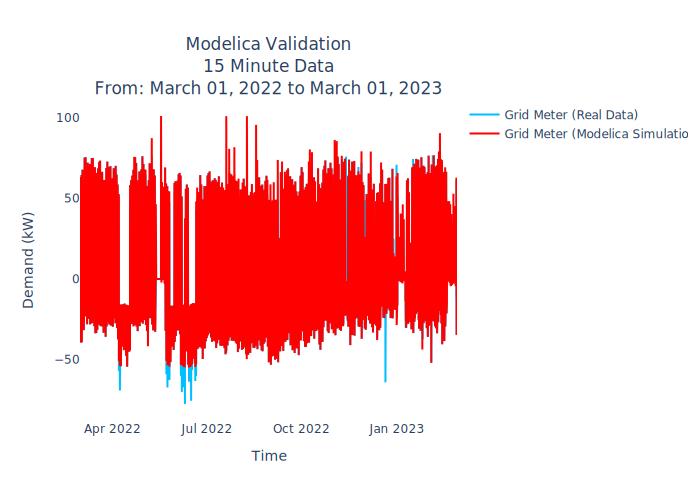
\includegraphics[width=1\linewidth]{Fig/ucr_15_Minute_Data_Mar_01_2022_to_Mar_01_2023}
			\caption{Whole Year Validation}
			\label{fig:ucr15minutedatamar012022tomar012023}
		\end{figure}
		
    \subsection{Solar Generation and Building Loads}
    	The solar power in our model is based on the historical solar data from our PV array. The HVAC loads and the regular building loads are represented separately in this model but utilize the same method; they both use historical real world power data to represent their load in the system. 
    \subsection{EV Charger Loads }
   		Our model also considers transportation loads in the form of EV chargers. The EV chargers are represented as two models: Level 2 EV chargers, and Level 3 EV chargers. While other loads follow a typical daily and yearly pattern, EV loads are different since they switch on and off. Our case study microgrid has four Level 2 chargers, so it can have four ``steps'' of 7.2 kW each, while there is only one ``step'' of 50 kW with the Level 3 chargers. To generate EV loads, we use a Poisson random generator to generate the number of charge sessions in a day, the arrival times, and charging durations based on real world data. 
		\begin{figure}[H]
			\centering
			\includegraphics[width=1\linewidth]{Fig/l2_avg_day_rand_poisson_1_hour_pdf}
			\caption{Probability Density Function of the Level 2 EV Charger Validation}
			\label{fig:l2avgdayrandpoisson1hourpdf}
		\end{figure}

%   		However, the number of sessions and duration is reduced to X and Y for the Level 3 charger.  
%		\begin{figure}[H]
%			\centering
%			\includegraphics[width=1\linewidth]{Fig/l2_avg_day_rand_poisson_1_hour}
%			\caption{Number of Real and Simulated Sessions}
%			\label{fig:l2avgdayrandpoisson1hour}
%		\end{figure}
		
		Historical data was collected from the Level-2 charger to determine the parameters for the Poisson random generator, following a typical daily charge pdf shown in Figure \ref{fig:l2avgdayrandpoisson1hourpdf}, and the power output of the Level 2 chargers in Figure \ref{fig:l2gpadpoissonjune}. 
		
			\begin{figure}[H]
				\centering
				\includegraphics[width=1\linewidth]{Fig/l2_g_pad_poisson_June}
				\caption{Level 2 Chargers Simulated Power Output}
				\label{fig:l2gpadpoissonjune}
			\end{figure}
%		\begin{figure}[H]
%			\centering
%			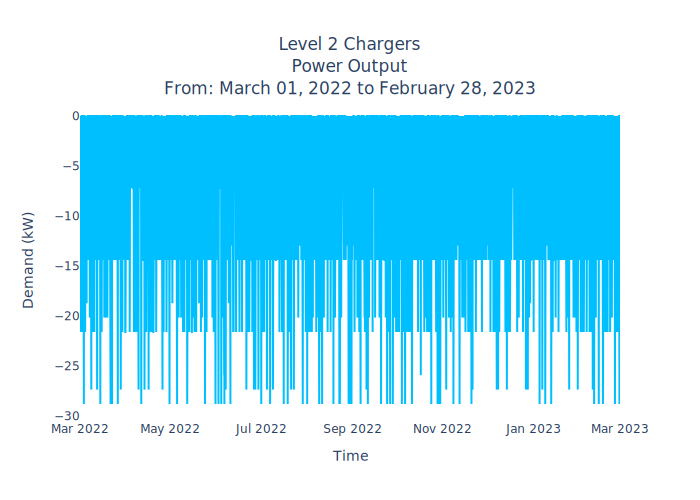
\includegraphics[width=1\linewidth]{Fig/ev_l2_po}
%			\caption{Level 2 Power Output}
%			\label{fig:evl2po}
%		\end{figure}
    
    \subsection{BESS and Peak Shaving}
    	The BESS is modeled as a battery connected to a bidirectional inverter. The BESS output is controlled by generated data from the control algorithm. The BESS output is computed in real-time by using a peak shaving algorithm utilizing  BESS SOC and the grid meter output. The algorithm charges the battery when excess solar power is exported to the grid, and the battery needs to be charged. Python code reads the net load from the grid  model and determines the amount of CO\textsubscript{2} being produced during that interval.  Algorithm \ref{alg:peakshavingflatrate} shows the peak shaving algorithm sufficient for flat rate demand response. 
%    	However,  for a TOU pricing structure, both energy and demand charges are assumed to be TOU rates with no additional flat rate demands. The TOU peak shaving algorithm is presented in Equation 1 with a simple objective to minimize the amount of power the microgrid pulls from the grid while accounting for energy and demand charges. The minimization objective is accomplished by optimizing for the summation of  TOU energy ($\Delta t \boldsymbol{\alpha}^{\boldsymbol{T}} \boldsymbol{P}^G$) and the maximums TOU demands ($\max \left(\boldsymbol{\beta}^{\text {On }} \boldsymbol{P}^G\right)+\max \left(\boldsymbol{\beta}^{\text {Mid }} \boldsymbol{P}^G\right)+\max \left(\boldsymbol{\beta}^{\text {Off }} \boldsymbol{P}^G\right)$). This algorithm is further described and validated in \cite{hasan2023universal},  \cite{hasan2021comprehensive} . \\
%%		\begin{figure}
%%			\centering
%%			\includegraphics[width=0.7\linewidth]{Fig/peak_shaving_flat_rate}
%%			\caption{Flat Rate Peak Shaving Algorithm Flowchart}
%%			\label{fig:peakshavingflatrate}
%%		\end{figure}
%			\normalsize
%			\footnotesize
%		\begin{equation} 
%			\min f\left(\boldsymbol{P}^G\right)=\Delta t \boldsymbol{\alpha}^{\boldsymbol{T}} \boldsymbol{P}^G+\max \left(\boldsymbol{\beta}^{\text {On }} \boldsymbol{P}^G\right)+\max \left(\boldsymbol{\beta}^{\text {Mid }} \boldsymbol{P}^G\right)+\max \left(\boldsymbol{\beta}^{\text {Off }} \boldsymbol{P}^G\right)
%		\end{equation}
%		\normalsize
%		subject to
%		$$
%		\begin{aligned}
%			& E_{t+1}^B=E_t^B+P_t^B \cdot \Delta t, \forall t \in \boldsymbol{T}^{\mathbf{t o t}} \\
%			& E^{B m i n} \leq E_t^B \leq E^{B m a x}, \forall t \in \boldsymbol{T}^{\mathbf{t o t}} \\
%			& P_t^B=P_t^{B+}-P_t^{B-}, \forall t \in \boldsymbol{T}^{\text {tot }} \\
%			& 0 \leq P_t^{B+} \leq \delta_t P^{B+\max }, \forall t \in \boldsymbol{T}^{\mathbf{t o t}} \\
%			& 0 \leq P_t^{B-} \leq\left(1-\delta_t\right) P^{B-\max }, \forall t \in \boldsymbol{T}^{\mathbf{t o t}} \\
%			& 0 \leq \delta_t \leq 1, \forall t \in \boldsymbol{T}^{\mathbf{t o t}} \\
%			& P_t^{B+}=\eta^{+} P_t^{S B}, \forall t \in \boldsymbol{T}^{\mathbf{t o t}} \\
%			& P_t^S=P_t^{S B}+P_t^{S L}, \forall t \in \boldsymbol{T}^{t o t} \\
%			& P_t^L=P_t^{S L}+P_t^{B L}+P_t^G, \forall t \in \boldsymbol{T}^{\text {tot }} \\
%			& P_t^{B L}=\eta^{-} P_t^{B-}, \forall t \in \boldsymbol{T}^{t o t} \\
%			& P_t^{S L} \geq 0, \forall t \in \boldsymbol{T}^{t o t}
%		\end{aligned}
%		$$

		\begin{algorithm}
			net\_load, SOC $\gets$ Modelica Data Output
			\uIf{if condition}{net\_load  <=   -15 kW and SOC > 20 \%  and net\_load  >=  -100 kW
				BESS\_inverter = -net\_load  - 15 kW
			}
			\uElseIf{net\_load  <= -100 kW and SOC > 20 \%}{
					BESS\_inverter = -100 kW
			}
			\uElseIf{net\_load  >=  0 kW and SOC < 90 \%  and net\_load  <=  100 kW}{ 
				 BESS\_inverter = -net\_load
			}
			\uElseIf{net\_load  >=  0 kW and SOC < 90 \%  }{
				 BESS\_inverter = 100 kW
			}
			\Else{
				BESS\_inverter = 0
			}
			\caption{Peak Shaving}
			\label{alg:peakshavingflatrate}
		\end{algorithm}

\section{Results}
	The charging setup is modified in OpenModelica for different layouts and scenarios. The scenarios are described in Table \ref{tab:scenarios}. Scenario 1 is the baseline case where only the building loads such as the air conditioners, appliances, and lights are connected to the grid. Scenario 2 is the case where a building installs four Level 2 and one Level 3 charger. Scenario 3 represents a transportation microgrid that has solar power and a BESS for peak shaving. Each scenario is run independently of each other, and the power outputs of the different components in the simulation are shown in Figure \ref{fig:scenariospoweroutputboxplot}. Scenario 1 and 2 are both constantly negative meaning they are constantly pulling power from the grid. Scenario 3 on the other hand is mostly positive or limited to -15, meaning it’s either exporting power to the grid or it’s consuming only 15 kilowatts. The reason for the 15 kilowatt floor is because with the utility companies electric rate a minimum of 15 kilowatts is charged for the demand, meaning that a zero demand microgrid will not make a financial difference for the user. While the peak shaving algorithm should limit the amount of power consumed at any time to be limited to 15 kilowatts, there are still some times when the BESS cannot supply the building with power. This happens when the BESS is too depleted, and there is little to no solar power to replenish it as shown in Figure \ref{fig:scenario3peakshaving}. The two main reasons for these events that happen are multiple cloudy days and electrical faults. During the winter months, most of the low solar power events occur since that is when most of the rain falls in southern California. Figures \ref{fig:scenariospoweroutputboxplot}, \ref{fig:0scnoutputrun2mar012022tomar312022}, and \ref{fig:4scnoutputrun2jul012022tojul312022} show box plots of the power output. Figure \ref{fig:scenariospoweroutputboxplot} is for the entire year while Figures \ref{fig:0scnoutputrun2mar012022tomar312022} and \ref{fig:4scnoutputrun2jul012022tojul312022} show selected months. The box plots show that all three figures mean and 75th percentile are almost identical at 15 kW. This implies that peak shaving is functioning correctly most of the time. However, the outliers show when the BESS fails to keep the power pulled from the grid at 15 kW. Just one outlier will change the demand charge for the entire billing month. In some months, the maximum demand peak of Scenario 2 and 3 are similar since they have the same load, but for most of the months, it is reduced significantly which is reflected on the reduced demand charges of the building. Each scenario’s power pulled from the grid is juxtaposed in Figure \ref{fig:netloadscenariocomparisonsummer}.The average of daily CO\textsubscript{2} emissions from each scenario is shown in Figure \ref{fig:emissionsscenariocomparison}. Scenario 2 with its increased charging events shows about a 26 \% increase of CO\textsubscript{2} emissions compared to Scenario 1. The CO\textsubscript{2} emissions from the transportation microgrid are lower than a conventional building even with the additional load coming from the EV chargers. The emissions and electric price amounts of each scenario are shown in Table \ref{tab:emissions}.
	\begin{table}[H]
		\caption{Simulated Scenarios of the UCR Microgrid using Different Layouts and Electric Pricing Structures}
		\tiny
		\begin{tabularx}{\linewidth}{X | l}
\toprule
 Scenario &  \\
\midrule
		1  & Standard Building with no EV Chargers\\
        2 & Standard Building with Level 2 and Level 3 Charging\\
        3 & Microgrid Building with Solar, 500 kWh BESS, Level 2, and Level 3 Charging\\
        4 & Microgrid Building with Solar, 1 MWh BESS, Level 2, and Level 3 Charging\\
\bottomrule
\end{tabularx}

		\normalsize
		\label{tab:scenarios}
	\end{table}
	
	\begin{figure}[H]
		\centering
		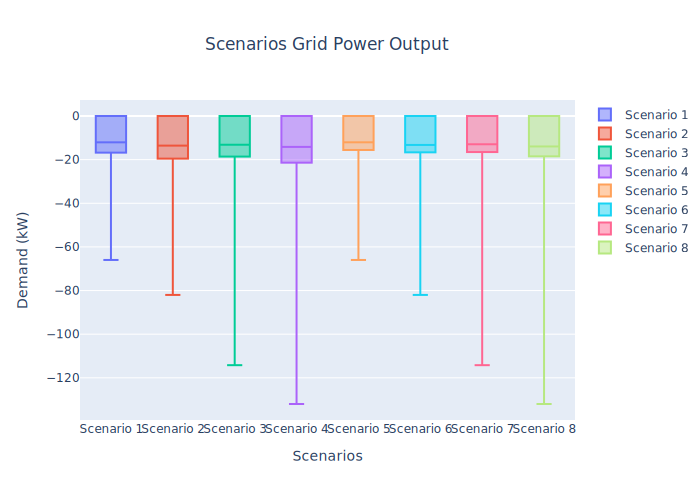
\includegraphics[width=0.9\linewidth]{Fig/scenarios_power_output_boxplot}
		\caption{Power measured from the meter}
		\label{fig:scenariospoweroutputboxplot}
	\end{figure}
	
	\begin{figure}[H]
		\centering
		\includegraphics[width=1\linewidth]{Fig/0_Scn_Output_Run_2_Mar_01_2022_to_Mar_31_2022}
		\caption{}
		\label{fig:0scnoutputrun2mar012022tomar312022}
	\end{figure}

	\begin{figure}[H]
		\centering
		\includegraphics[width=1\linewidth]{Fig/4_Scn_Output_Run_2_Jul_01_2022_to_Jul_31_2022}
		\caption{}
		\label{fig:4scnoutputrun2jul012022tojul312022}
	\end{figure}
	
%	\begin{figure}[H]
%		\centering
%		\includegraphics[width=0.9\linewidth]{Fig/scenarios_mg_load_output_boxplot}
%		\caption{Load of all the microgrid components}
%		\label{fig:scenariosmgloadoutputboxplot}
%	\end{figure}
	



    
	\begin{figure}[H]
		\centering
		\includegraphics[width=1\linewidth]{Fig/net_load_scenario_comparison_summer_run_2}
		\caption{Summer Net Load Scenario Comparison}
		\label{fig:netloadscenariocomparisonsummer}
	\end{figure}
	
	
	\begin{figure}[H]
		\centering
		\includegraphics[width=1\linewidth]{Fig/scenario_3_peak_shaving}
		\caption{}
		\label{fig:scenario3peakshaving}
	\end{figure}
	
	\begin{figure}[H]
		\centering
		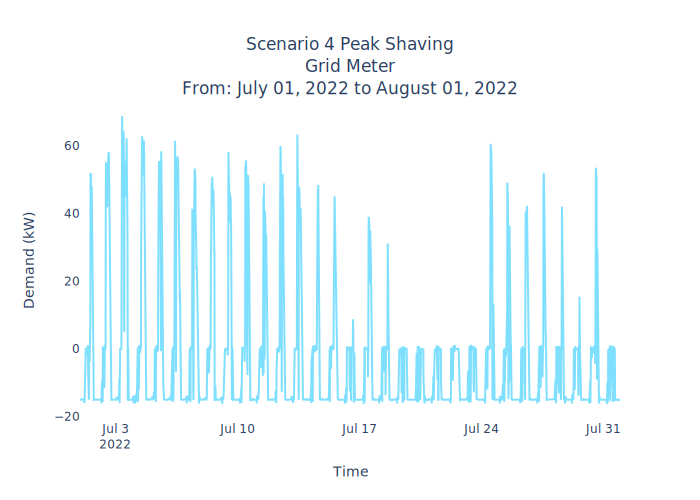
\includegraphics[width=1\linewidth]{Fig/scenario_4_peak_shaving}
		\caption{}
		\label{fig:scenario4peakshaving}
	\end{figure}

	\begin{figure}[H]
		\centering
		\includegraphics[width=1\linewidth]{Fig/emissions_scenario_comparison_run_2}
		\caption{Microgrid  CO\textsubscript{2} Emissions Outputs Averages During Times of Day}
		\label{fig:emissionsscenariocomparison}
	\end{figure}
	
	\begin{table}[H]
		\caption{Microgrid Utility Prices and CO\textsubscript{2} Emissions Output under Different Pricing Scenarios and Pricing Structures}
		\tiny
		\centering
		\input{Table/kw_kwh_CO2_run_3.tex}
		\normalsize
		\label{tab:emissions}
	\end{table}
	
	\section{Conclusion}
		Transportation microgrids are an innovative solution for reducing the electric costs and emission levels of an EV charging setup. A comparative analysis of different scenarios shows that a transportation microgrid can offer significant savings and CO\textsubscript{2} over a conventional system. For a 100 kW 500 kWh transportation microgrid system, the annual savings are estimated to be \$8,000 a year or \$80,000 over a 10-year battery lifetime, even with additional demand from EV chargers. Compared to a building that installs EV chargers without a microgrid, the annual savings are even more substantial, reaching \$27,000 a year or \$270,000 over a 10-year battery lifetime. This implies that the transportation microgrid can triple the savings from switching from a conventional building. Moreover, the transportation microgrid can reduce the CO\textsubscript{2} emissions by more than 50\% compared to the conventional building and by about 67\% compared to the scenario where the microgrid does not supply the building with clean energy. Therefore, the user has a strong economic and environmental incentive to adopt a transportation microgrid. However, increasing the battery capacity does not necessarily improve the performance of the microgrid. As shown in the month of July in Figures \ref{fig:scenario3peakshaving} and \ref{fig:scenario4peakshaving}, doubling the battery capacity can eliminate some peaks from a couple of cloudy days, but the additional savings of \$2,000 per year do not justify the cost of the extra capacity. Lastly, a 15 kW demand price floor has a negative impact on CO\textsubscript{2} emissions, as it discourages the user from maintaining the net load at zero in a peak shaving setup.
	\section{Future Works}
		  Future research will explore different, more advanced control strategies to optimize the electric costs and CO\textsubscript{2} emissions of the transportation microgrid. These strategies will include preventing users from charging during high peak times, maximizing the use of the clean energy produced by the solar panels, and minimizing the power drawn from the grid during high CO\textsubscript{2} times. The effect of the new net energy metering policy in California on the value of the BESS system will also be assessed.
%		\nocite{*}
		\bibliographystyle{IEEEtran}
		\bibliography{cite}
		
\end{document}
